\documentclass[tikz,border=7pt]{standalone}
\usepackage[T1]{fontenc}
\usepackage[utf8]{inputenc}
\usetikzlibrary{positioning}
\begin{document}
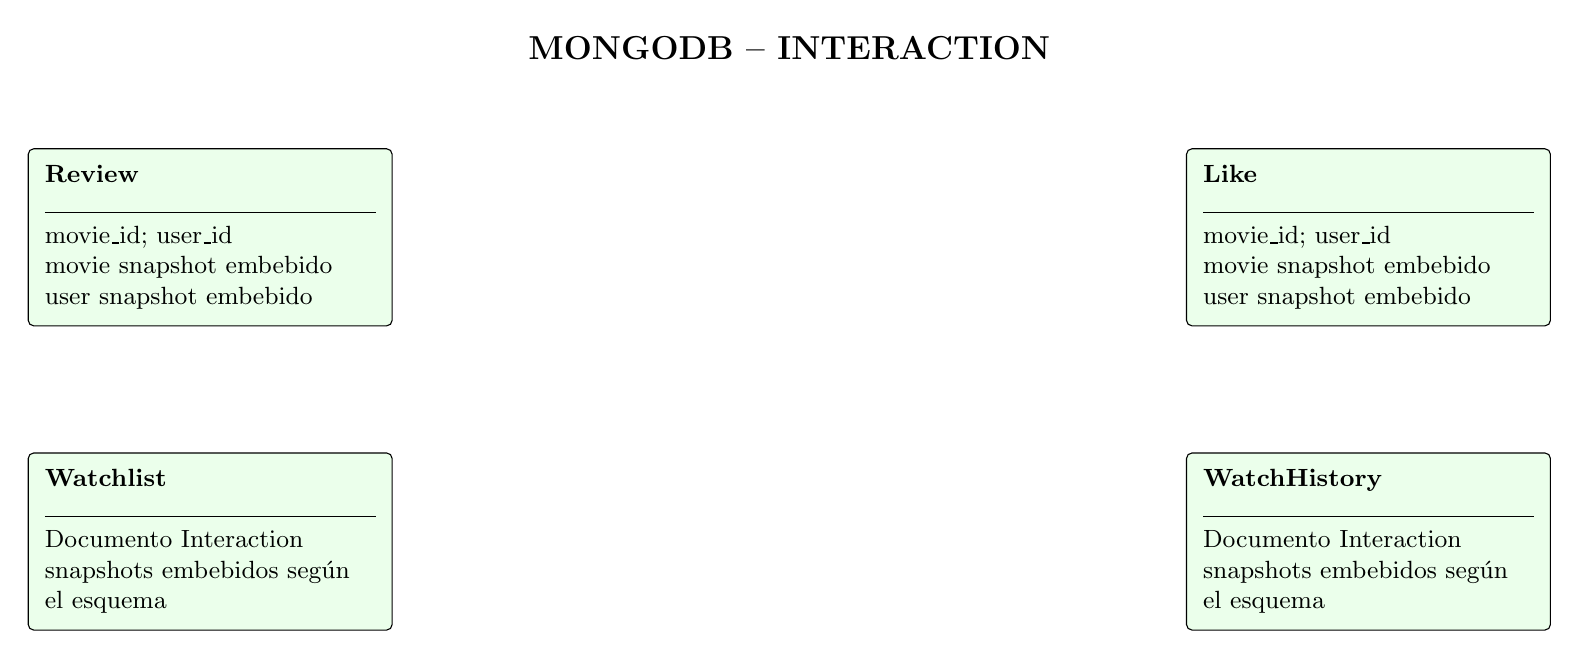
\begin{tikzpicture}[font=\small, entity/.style={draw, rounded corners=2pt, align=left, text width=4.2cm, inner sep=6pt, fill=green!8}, heading/.style={font=\bfseries\large}]
\node[heading] (title) {MONGODB -- INTERACTION};
\node[entity, below left=10mm and 16mm of title] (review) {\textbf{Review}\\\rule{4.2cm}{0.3pt}\\movie\_id; user\_id\\movie snapshot embebido\\user snapshot embebido};
\node[entity, below right=10mm and 16mm of title] (like) {\textbf{Like}\\\rule{4.2cm}{0.3pt}\\movie\_id; user\_id\\movie snapshot embebido\\user snapshot embebido};
\node[entity, below=16mm of review] (watchlist) {\textbf{Watchlist}\\\rule{4.2cm}{0.3pt}\\Documento Interaction\\snapshots embebidos según el esquema};
\node[entity, below=16mm of like] (history) {\textbf{WatchHistory}\\\rule{4.2cm}{0.3pt}\\Documento Interaction\\snapshots embebidos según el esquema};
\end{tikzpicture}
\end{document}
